\section{V3}
\vspace{-0.5cm} 
    \begin{minipage}{9cm}
        \subsection{Halbleiter Speicher} 
        \textbf{Zentraler Speicher}
        \begin{itemize}
            \item direkt am Bussystem angeschlossen
        \end{itemize}
        \textbf{Peripherer Speicher}
        \begin{itemize}
            \item über I/O-Schnittstelle angeschlossen
        \end{itemize}
    \end{minipage}
    %
    \begin{minipage}{0.5cm}
    	\ \
    \end{minipage}
    %
    \begin{minipage}{9cm}
    	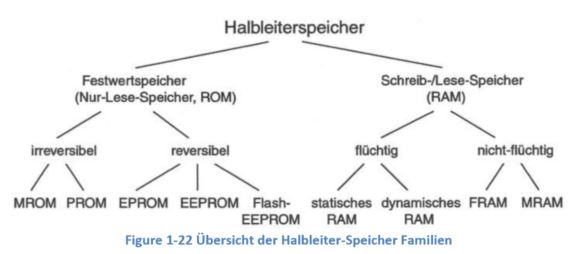
\includegraphics[width=9cm]{images/halbleiterfam}
    \end{minipage}
 
\begin{multicols}{2}
    \subsubsection{ROM-Festwertspeicher}
    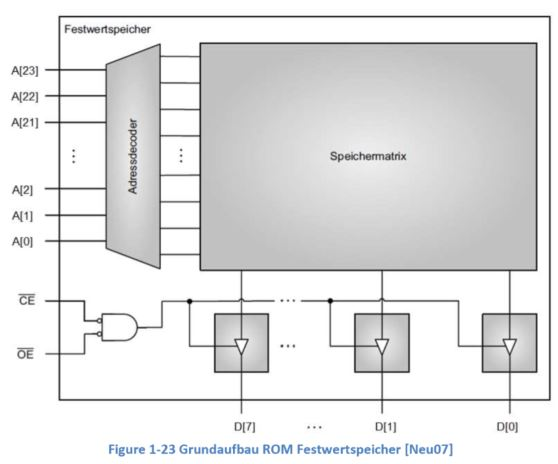
\includegraphics[width=8cm]{images/ROM}
    
    \subsubsection{RAM-Speicher-/Lese-Speicher}
    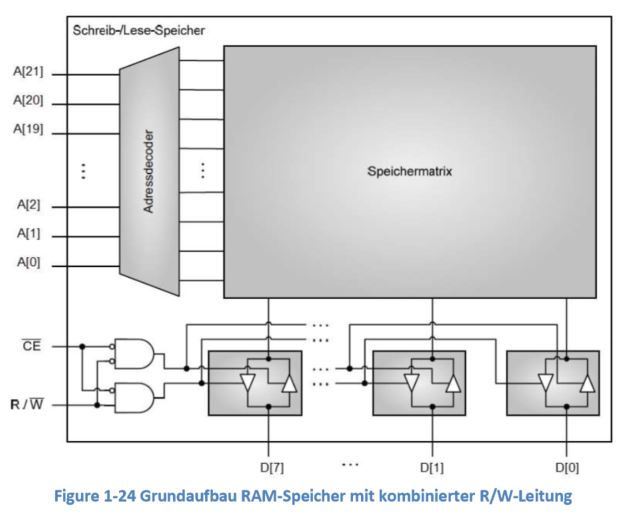
\includegraphics[width=8cm]{images/RAM}
\end{multicols}

\subsection{Speicherorganisation}
\begin{minipage}{9cm}
	\subsubsection{Little/Big Endian}
    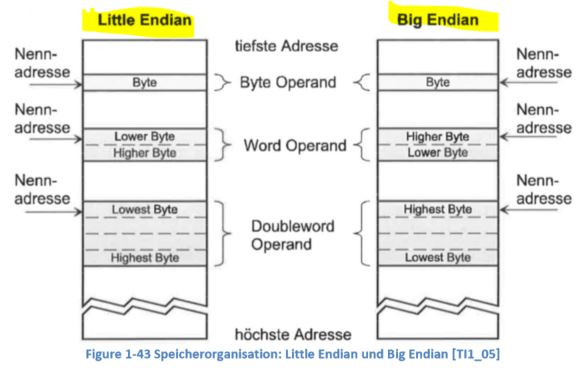
\includegraphics[width=8cm]{images/LittleBigEndian}
    
    Der ARM Cortex verwendet standardm"assig \textbf{Little Endian} f"ur die Speicherorganisation. 
\end{minipage}
%
\begin{minipage}{0.5cm}
	\-\
\end{minipage}
%
\begin{minipage}{9cm}
	 \subsubsection{I/O - Schnittstelle}
    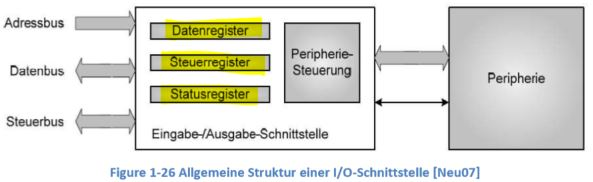
\includegraphics[width=8cm]{images/IOSchnittstelle}
    
    \textbf{Datenregister}
    \begin{itemize}
    	\item enthalten die zu verarbeitenden Daten
    \end{itemize}
    \textbf{Steuerregister}
    \begin{itemize}
    	\item dienen zur Konfiguration der Ein-/Ausgabe Schnittstelle
    \end{itemize}
    \textbf{Statusregister}
    \begin{itemize}
    	\item signalisieren den Zustand der Ein-/Ausgabe Schnittstelle
    \end{itemize}
\end{minipage}
 
\subsubsection{Speicherraumadressierung}
\begin{minipage}{11cm}
	\includegraphics[width=11cm]{images/Speicherraumadressierung}
\end{minipage}
%
\begin{minipage}{0.5cm}
	\-\
\end{minipage}
%
\begin{minipage}{7cm}
	\textbf{Isolierte Adressierung}
	\begin{itemize}
		\item Gesamter Adressraum steht verschiedener Bl"ocken zur Verf"ugung
		\item Bl"ocke werden mit einem Steuersignal ausgew"ahlt
	\end{itemize}
	\textbf{Memory-Mapped I/O (Cortex M3)}
	\begin{itemize}
		\item Verschiedene Bl"ocke werden in einen Adressraum eingebettet
		\item Ben"otigt eine Adresskodierung
	\end{itemize}
\end{minipage}

\newpage
\subsection{Busanschluss und Adressverwaltung}
Eine Adressverwaltung hat verschiedene Aufgaben zu erf"ullen:
\begin{itemize}
	\item Jede Adresse spricht nur einen einzigen Speicher- oder I/O-Baustein an.
	\item Adressraum m"oglichst gut ausn"utzen
	\item Adressr"aume von Speicherbausteinen m"ussen l"uckenlos aufeinander folgen.
	\item Jeder interne Speicherplatz bzw. jedes Register erscheint unter einer eigenen Adresse im Systemadressraum.
\end{itemize}

\subsubsection{Adresskodierung}
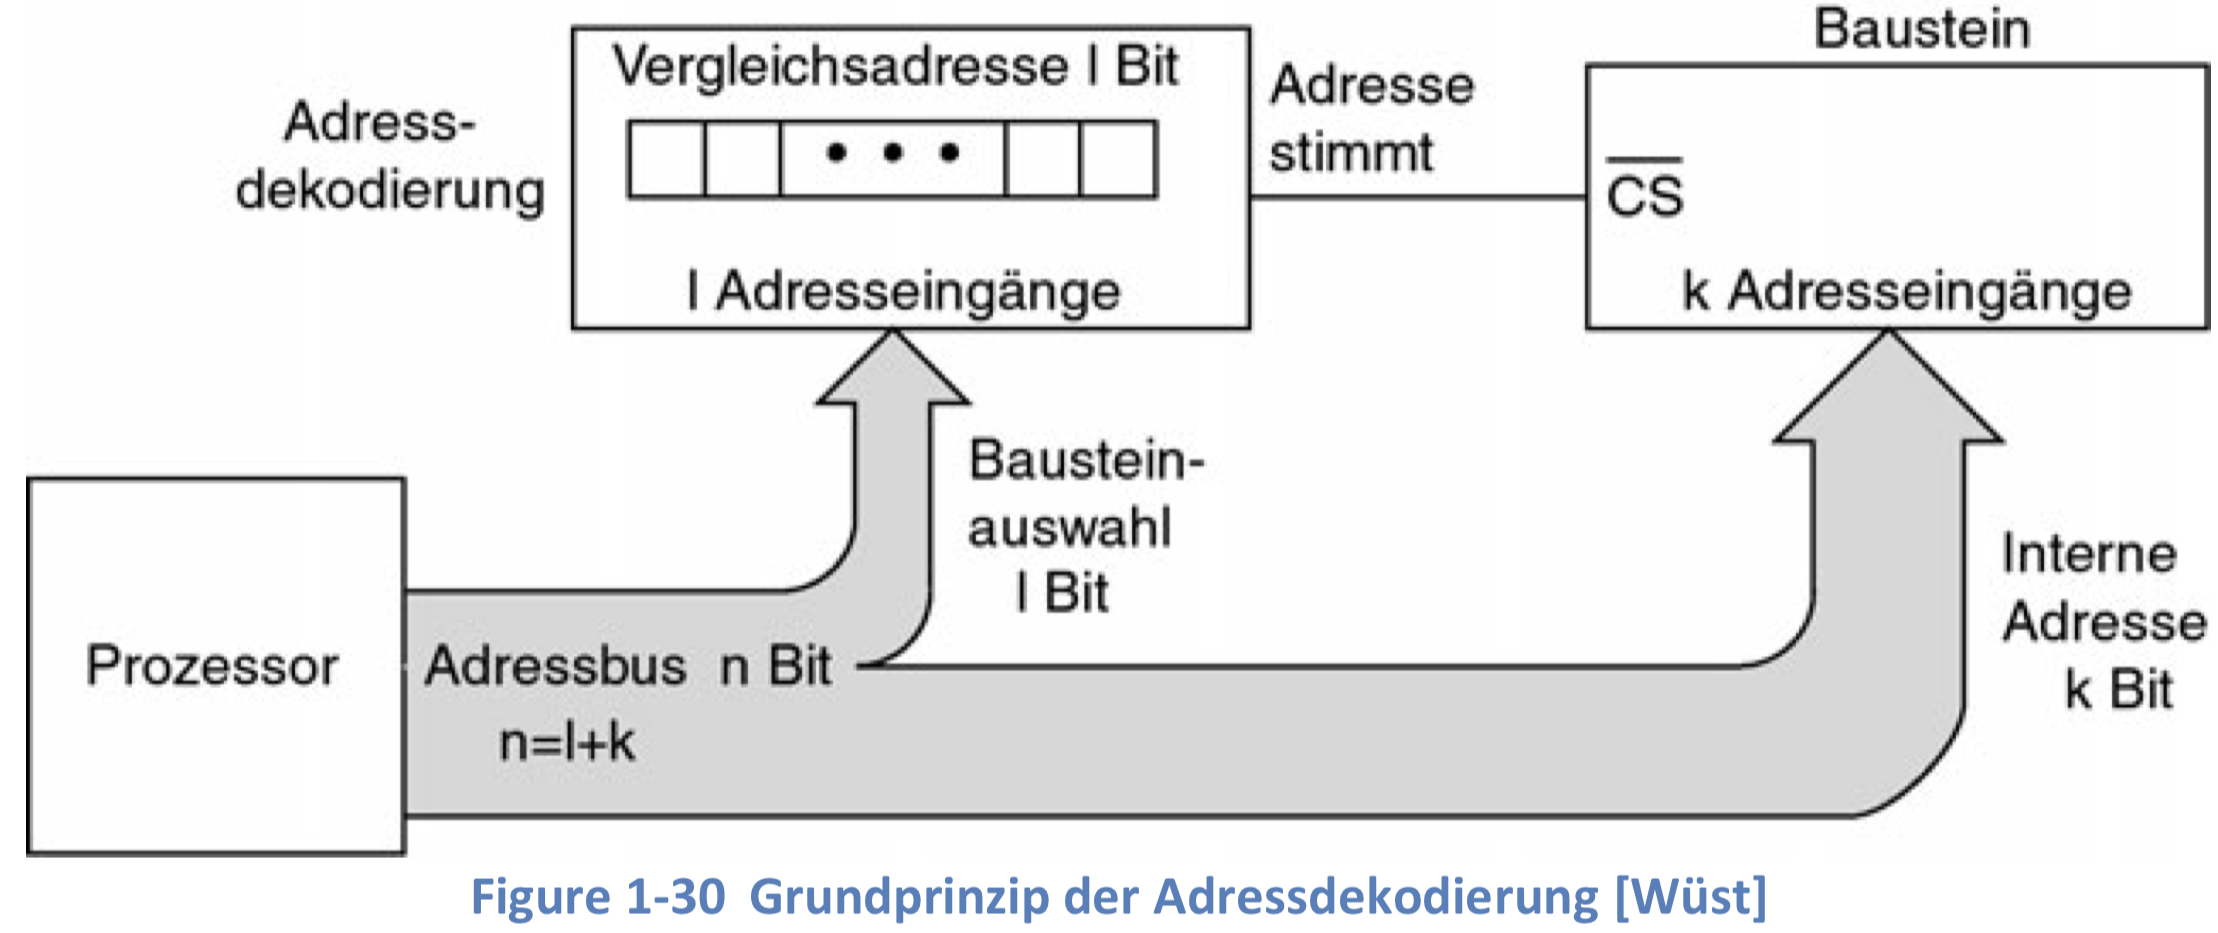
\includegraphics[width=14cm]{images/Adressverwaltung}\\
Der Kernpunkt der Adresskodierung ist die Teilung des Adressbuses. Dabei werden die \textit{k} niedrigsten Adressleitungen direkt an die Adresseing"ange des Bausteines gef"uhrt und dienen zur Auswahl des gew"unschten internen Speicherplatzes oder Registers. Die n"achstfolgenden \textit{l} Adressleitungen werden zur Adresskodierung auf einen Adressdekoder gef"uhrt.
\clearpage
%============================================






















